% !TEX encoding = UTF-8 Unicode
% !TEX root = project.tex

\section{Related Work}
\label{sec:related}

In the past many authors and research institutes have focused their research work on finding defects and dependency graphs. \\

One of the most significant work was done by Thomas Zimmerman et al.~\cite{zimmermann2008predicting}, who tried to predict defects using network analysis on dependency graphs. The authors claimed that models using network analysis on dependency graphs to find defects proved to have better recall of around 10\% points higher than other models that used complexity metrics. Also, they proved that dependency graphs can help in finding around 60\% of critical areas, twice as identified by any other counterparts. Authors in this paper used, along with many other algorithms, Bron-Kerbosch's algorithm, which uses size of clique to determine the number of defects in that region. Their claim is that as the size of the clique grows, its binaries become more defect-prone. Finally, they found that the average number of defects increases with the size of the clique a binary resides in. Figure~\ref{fig:relatedwork} and Figure~\ref{fig:relatedwork1} shows a glimpse of what the Bron-Kerbosch is aimed at and how the results will look like, respectively. In our study and implementation, we tried to implement Bron-Kerbosch algorithm, but we could not get any meaningful results on the projects that we tried.

\begin{figure}[h!]
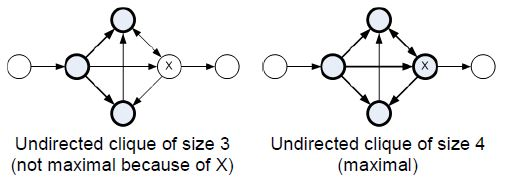
\includegraphics[width=8cm]{relatedwork}
\caption{Undirected cliques}
\label{fig:relatedwork}
\end{figure}

\begin{figure}[h!]
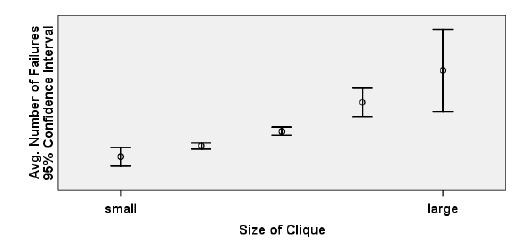
\includegraphics[width=8cm]{relatedwork1}
\caption{Defect-Proneness of binaries in cliques}
\label{fig:relatedwork1}
\end{figure}

Our evaluation section follows similar steps as implemented in the paper that we just mentioned. In our evaluation, we performed an experimental study that attempted to use 2 major algorithms, Kosaraju-Sharir and Bron-Kerbosch's algorithm to find the defect-prone areas in the source repositories. Although we were unsuccessful with Bron-Kerbosch algorithm, we managed to get some results out of the implementation of Kosaraju-Sharir algorithm. Later, the Noodlr tool shows the strongly connected components on the graph obtained using the Kosaraju-Sharir algorithm. Results are discussed in more detail in the evaluation section (Section~\ref{sec:finding}). \\

Another study~\cite{bhattacharya2012graph} done by the researchers of the Department of Computer Science, University of California - Riverside discusses the recent advancements in analysis of graph topology to make the understanding of software evolution more clear. Also, they tried to create predictors that can help in software development and maintenance. In this study, they demonstrated how graph based analysis can be used in software evolution by estimating bug severity, prioritizing re-factoring efforts and also predict defect-prone releases. As compared to this, Noodlr also helps in various stages of software development including development, testing and maintenance stages which are discussed in detail in Practical Applications (Section~\ref{sec:practical}). \\

At 34\textsuperscript{th} Euromicro Conference Software Engineering and Advanced Applications~\cite{turhan2008software}, a paper was published on predicting software defects using Call Graph Based Ranking (CGBR). In this study, authors claimed to use static call graph based ranking along with a defect prediction model. Though the results show that CGBR framework could get the same number of defective modules as other counterparts, it produced very low false alarm rates. In their evaluation study, they proved that testing process can be improved by 23\% through CBGR framework. This study proposed a novel combination of the static code attributes (SCA) and architectural structure of software to make predictions about defect content of software modules.\\

A slight variant of ~\cite{turhan2008software} in this area is presented in~\cite{eichinger2008mining}. Authors of the paper~\cite{eichinger2008mining} tried to solve the problem of automating the discovery of non-crashing occasional bugs. They claimed that mining of weighted call graphs of program executions could be a good way to automate this. In their model, they proposed a novel reduction technique for call graphs which introduces edge weights on each link. Then this weighted graph is used for analysis to find bugs. Evaluation provided some bugs which were not detected by any other previous studies and even the precision of finding localised bug doubled compared to any other prior studies.\\

A recent study on telecommunication industry~\cite{turhan2009data} that includes mining source code using data mining techniques for locating software bugs was presented in Elsevier 2009 conference. The paper focused on similar objectives like our paper to help managers in resource allocation and testing by predicting defect-prone areas in large-sized projects. They followed an approach similar to the CBGR methodology as discussed in ~\cite{turhan2008software}. Results of this paper suggested that, at least 70\% of the defects can be detected by inspecting only 6\% of the code using a Naive Bayes model and 3\% of the code using CGBR framework.\\

Now, in the next section, we look at the actual software implementation of the frontend and the backend. We explain how the above mentioned algorithms are used in the software as well as how the data is presented in the Noodlr interface, which is our web-based tool.

